%%%%%%%% ICML 2020 EXAMPLE LATEX SUBMISSION FILE %%%%%%%%%%%%%%%%%
\documentclass{article}

% Recommended, but optional, packages for figures and better typesetting:
\usepackage{microtype}
\usepackage{graphicx}
\usepackage{subfigure}
\usepackage{booktabs} % for professional tables

% hyperref makes hyperlinks in the resulting PDF.
% If your build breaks (sometimes temporarily if a hyperlink spans a page)
% please comment out the following usepackage line and replace
% \usepackage{icml2020} with \usepackage[nohyperref]{icml2020} above.
\usepackage{hyperref}

% Attempt to make hyperref and algorithmic work together better:
\newcommand{\theHalgorithm}{\arabic{algorithm}}

% Use the following line for the initial blind version submitted for review:
% \usepackage{icml2021}
\usepackage[accepted]{icml2021}

% If accepted, instead use the following line for the camera-ready submission:
%\usepackage[accepted]{icml2020}

\usepackage{times}
\usepackage{epsfig}
\usepackage{amsmath}
\usepackage{amssymb}
\usepackage{comment}
\newcommand{\nop}[1]{}

% Listings for code snippets.
\usepackage{listings}
\lstset{frame=tb,
  language=Python,
  aboveskip=3mm,
  belowskip=3mm,
  showstringspaces=false,
  columns=flexible,
  basicstyle={\small\ttfamily},
  numbers=none,
  numberstyle=\tiny\color{gray},
  keywordstyle=\color{blue},
  commentstyle=\color{dkgreen},
  stringstyle=\color{mauve},
  breaklines=true,
  breakatwhitespace=true,
  tabsize=3
}

% The \icmltitle you define below is probably too long as a header.
% Therefore, a short form for the running title is supplied here:
\icmltitlerunning{Multi-Armed Bandits for Optimizing New Peers in Peer-to-Peer Networks}

\begin{document}

\twocolumn[
\icmltitle{Multi-Armed Bandits for Optimizing New Peers in Peer-to-Peer Networks}

% It is OKAY to include author information, even for blind
% submissions: the style file will automatically remove it for you
% unless you've provided the [accepted] option to the icml2020
% package.

% List of affiliations: The first argument should be a (short)
% identifier you will use later to specify author affiliations
% Academic affiliations should list Department, University, City, Region, Country
% Industry affiliations should list Company, City, Region, Country

% You can specify symbols, otherwise they are numbered in order.
% Ideally, you should not use this facility. Affiliations will be numbered
% in order of appearance and this is the preferred way.
% \icmlsetsymbol{equal}{*}

\begin{icmlauthorlist}
\icmlauthor{Oscar Sandford}{to}
\icmlauthor{Shawn Nettleton}{to}
\end{icmlauthorlist}

\icmlaffiliation{to}{Department of Computer Science, University of Victoria, Victoria, Canada}

\icmlcorrespondingauthor{Oscar Sandford}{oscarsandford@uvic.ca}
\icmlcorrespondingauthor{Shawn Nettleton}{shawnnettleton@uvic.ca}

% You may provide any keywords that you
% find helpful for describing your paper; these are used to populate
% the "keywords" metadata in the PDF but will not be shown in the document
\icmlkeywords{Machine Learning, ICML}

\vskip 0.3in
]

% this must go after the closing bracket ] following \twocolumn[ ...

% This command actually creates the footnote in the first column
% listing the affiliations and the copyright notice.
% The command takes one argument, which is text to display at the start of the footnote.
% The \icmlEqualContribution command is standard text for equal contribution.
% Remove it (just {}) if you do not need this facility.

\printAffiliationsAndNotice{}  % leave blank if no need to mention equal contribution
%\printAffiliationsAndNotice{\icmlEqualContribution} % otherwise use the standard text.

\begin{abstract}
Write this last (fewer than 300 words). The completed document should be 5-9 pages.
\end{abstract}

%-------------------------------------------------------------------------------
% Problem, why it is important/interesting, and the plan for the approach.
\section{Introduction}
Peer-to-peer computer networks create a unique environment for content distribution wherein the integrity of the system is not compromised by the failure of 
a single, centralized node in the network. According to \cite{p2p_def}, true peer-to-peer systems require peers to be mutually directly accessible (without 
intermediate entities), as well as the network state or quality of service being preserved in the advent of a peer being removed from the network, for any 
reason.

The requirements for peer-to-peer networks in different application domains vary. However, new peers that are directly accessing the server for the first time 
have no information on the network state. New peers therefore cannot be held accountable to preserve the network state and its content if other nodes disconnect. 
It is essential that this new peer is fed the relevant data as fast as possible in order to fulfill both the requirements of a true peer-to-peer environment, as 
well as any necessary quality of service targets. With the added volatility of a dynamic network setting, the rate at which a new peer can be brought "up to speed" 
becomes far more crucial.

In this study, we abstract the new peer scenario described above as a reinforcement learning problem with multi-armed bandits. The multi-armed bandit (MAB) problem 
involves $k$ slot machines (slot machines are sometimes called one-armed bandits) which pay out reward values according to an internal distribution, of which the agent 
is not aware (note that some MAB variations may relax these constraints). The goal is to pick a strategy to learn which arms pay out the most in order to to maximize 
total reward over a set number of rounds \cite{mab_algos}. 

We consider various algorithms to solve the multi-armed bandit problem, and a select few are implemented in order to evaluate their efficacy against this problem. 
Related literature is surveyed in order to compare our work with solutions to similar problems and verify the validity of our results. Formulation of this challenge 
as a reinforcement learning problem precedes an explanation of the approach and a discussion of the results. The following section contains a survey of related work 
concerning the application of multi-armed bandits to computer networking problems.

%-------------------------------------------------------------------------
% Related work section. Discuss relevant literature.
\section{Related Work}

Multi-armed bandits serve as a useful abstraction for optimization problems that require decision making with reward outcomes that are initially unknown. In a study 
on cognitive radio networks \cite{qos_selection_mab}, secondary user (SU) nodes select a single channel for information exchange at one time, with no knowledge about 
channel quality or availability. The authors use a variation on the upper confidence bound (UCB) algorithm, namely QoS-UCB. Their scenario is called "restless", 
meaning that the states of the arms can fluctuate over time, affecting their internal distrubtions and the resulting payouts.

The task of wireless network selection, with the goal of maximizing perceived quality for the end user, is handled by extending the bandit model to be more flexible 
\cite{muMAB_wireless}. In this formulation, the agent can take one of two actions (which can span multiple time steps): measure or use. The difference is that 
measurement allows only evaluation, whereas using adds exploitation. Measuring takes less time than using, which can span a set number of time steps. Results showed 
that the choice of algorithm depended on the payout distributions. Conservative UCB1 is useful when arm rewards are similar, MLI when one arm is clearly better. 
More aggressive algorithms like POKER can lead to low regret but high variability, and are therefore less reliable \cite{muMAB_wireless}.

Anver and Mannor share methods for multiple multi-armed bandit agents, coordinating with each other and learning stochastic network conditions, which may vary between 
users \cite{multiuser_mab}. Their problem formulation is similar to our intentions, but with the agent transmitting instead of receiving. Further, they bound their rewards 
on the interval $[0,1]$. The problem with this reward formulation when it comes to receiving is that, while outward transmission speed or success may be measureably bounded, 
reception rate is not necessarily bounded. In fact, there may be conditions when the end receiver does not have the resources to unpack the transmission packages in time, 
and will become congested. This paper uses techniques to deal with collisions when two or more users transmit in a single channel \cite{multiuser_mab}. In our problem, we 
are only operating with unicast in a channel selected by the requesting peer. A last thing of note is Anver and Mannor's use of UCB in the channel ranking part of their 
algorithm selection.

Another paper surveys resource scheduling with multi-armed bandits in wireless networks \cite{mab_wireless_scheduling_survey}. They mention that $\varepsilon$-greedy, an 
algorithm that balancing exploration and exploitation, has shortcomings in its "pure" randomness, and does not take into account confidence intervals on the reward estimates 
of each arm. UCB exploits this, and also tapers off exploration over time. The authors make the distinction between single- and multi-player multi-armed bandits (SMAB and 
MMAB), where the former involves a single agent operating the bandit selection mechanism. SMAB have applications in our single peer leeching scenario, as well as centralized 
network algorithms. MMAB often involve distributed selection that sacrifices independence for synchronization overhead \cite{mab_wireless_scheduling_survey}.

Similarly Eshcar Hillel \textit{et al}, explore how $k$ players collaborate to identify an $\varepsilon$-optimal arm in a MAB setting, and determine communicating only
once players are able to learn at a rate of $\sqrt{k}$ times faster than a single player \cite{mab_dist_exploration}. This methodology may prove useful as the number of 
peers within the network fluctuates or quality of service changes. 

Multi-armed bandit problems have been gaining significant attraction. However, little effort has been devoted to adapting existing bandit algorithms to specific architectures 
such as peer-to-peer network environments \cite{gossip_based_distrivuted_stochastic}. This paper successfully implements the $\varepsilon$-greedy stochastic algorithm to a 
peer-to-peer network environment, scaling with the size of network, achieving a linear speedup in terms of the number of peers, and preserving the asymptotic behaviour of the 
standalone version. They also present a heuristic which has a lower network communication cost which may prove helpful with adapting other related works. 

Scenarios of distributed clustering have shown to be promising at solving MAB problems within peer-to-peer networks \cite{dist_clustering_p2p}. There are two setups in 
particular, the first where all peers are solving the same problem and second where a cluster of peers solve the same problem within each cluster. This has shown to achieve 
an optimal regret rate, defined as the expected difference between the reward sum associated with an optimal strategy and the sum of the collected rewards. 
%cut: We hope to adapt these works within our approach.

Competition amongst peers is inevitable within the peer-to-peer network environment, especially when peers are trying to stay up to date. Managing this competition can be 
difficult given its unpredictable nature. Miao Yang \textit{et al}, develop an online learning policy based on top of a MAB framework to deal with peer competition and 
delayed feedback \cite{p2p_offloading_with_delayed_feedback}. However, their work is with relation to fog networks (FN), a decentralized computing infrastructure between 
the data source and the cloud. We aim to utilize some of their understandings while tackling the peer-to-peer network scenario. 

The work done within \cite{p2p_net_sender_scheduling} showcases new considerations for not only optimizing data rate transmissions in wireless peer-to-peer networks but also 
minimizing power consumption. Similar limitations are becoming popular when analyzing the use of graphical processing units (GPUs) such as the work within \cite{gpu_eng}. As 
more domain problems are aspiring for optimal performance it is important to recognize new aspects such as power consumption. 



%-------------------------------------------------------------------------
\section{Problem Formulation}

Although we have so far informally hinted at the application of multi-armed bandits to this problem, this section is devoted to formalizing that congruence.

Consider the setting of a peer-to-peer network wherein a new peer joins with the intent to be brought "up to speed" with the rest of the network as soon as 
possible (i.e. download all the data in the network from other peers). However, the new peer does not know the network speeds of its seeds, just how much data 
it receives over time when it chooses a peer and receives data from them for one (or more) time step(s). The reward is the average number of bytes received across 
the number of time steps spent on that action. We will assume that data packets are UDP datagrams.

\begin{center}
    Do not confuse timesteps with steps (or rounds) in the algorithm. Multiple time steps can happen during a single round, because \emph{a step is when the agent makes a 
decision for a given number of time steps}. We use steps and rounds interchangeably. Keep this distinction in mind in the context of this study.
\end{center}

The agent should aim to choose the peer that is transmitting the fastest. However, consider that network speeds may change, and the optimal seed to leech from will 
not always be the best. We call this a "restless" scenario. We simulate these dynamics by assigning each peer a set of possible states, as well as a transition matrix 
of probabilities to transition from one state to another at every time step. In this sense, every peer is running its own Markov process in the background, irrespective 
of the agent's action.

This scenario can be solved with a multi-armed bandit approach. Each peer is considered as an "arm" in the multi-armed bandit algorithm. The agent will choose to 
"pull an arm" and receive reward for a certain number of \emph{time steps} (by default 1). During every time step, the network dynamics shift, and each arm may 
transition to another one of its states (regardless of if it was the arm selected or not). Naturally, this creates greater variance in average reward payout, which 
serves to simulate the noise present in real-world network systems. 

Previous studies \cite{multiuser_mab,gossip_based_distrivuted_stochastic,p2p_offloading_with_delayed_feedback} consider peer-to-peer networks where the peers communicate 
or compete with one another. However, our scenario assumes no information about peers is initially present on the hardware of the new peer, and that transmitting this 
information ahead of the vital data packets should not be a priority. Therefore, the "trial-and-error" methodology of multi-armed bandit agents fits the learning 
requirements under these constrained conditions.


%-------------------------------------------------------------------------
% Algorithms we will use and develop (e.g. eps-greedy, UCB, and more). Implementation details, pseudocode here.
\section{Approach}

% \cite{mab_algos_1} - theoretical guarantees vs practical results of algorithms.

In this section we briefly outline each algorithm considered, and present our approach for generating test scenarios and measuring the algorithms' efficacy against the 
new peer update task within a small set of hyperparameters. The accompanying source code for our work is maintained on 
GitHub\footnote{https://github.com/oscarsandford/network-bandit}.

\subsection{Algorithms} \label{sec:algos}

The most common baseline algorithm applied to multi-armed bandit problems is called $\varepsilon$-greedy. $\varepsilon$-greedy takes a single hyperparameter $\varepsilon$ 
that dictates the probability of exploration (i.e. choosing a random arm from the possible selections), with $1-\varepsilon$ being the probability of choosing the optimal 
arm based on the average rewards so far. We make use of $\varepsilon$-greedy, as well as some of its variants in this study. 

Firstly, $\varepsilon$-first is an $\varepsilon$-greedy strategy where only exploration is done for the first $T\varepsilon$ rounds, and pure exploitation 
is done during the remaining rounds. $T$ is the number of rounds (also called steps) per run \cite{mab_algos}. This forced exploration means peak rewards will be delayed, 
but more learning is attained as a result.

In addition, $\varepsilon$-decreasing is another $\varepsilon$-greedy variant wherein the initial $\varepsilon$ value $\varepsilon_0$ is decreased over the number of rounds 
completed. More specifically, the probability of exploration at time $t$ is given by $\varepsilon_t = min\{ 1, \frac{\varepsilon_0}{t}\}$ where $\varepsilon > 0$. Values for 
$\varepsilon_0$ are typically not on the interval $[0,1]$, instead values like $1.0$, $5.0$, and $10.0$ are used \cite{mab_algos}.

SoftMax (also called Boltzmann Exploration) makes action decisions based on \emph{probability matching} methods \cite{mab_algos}. Each arm $a$ of $k$ arms holds an associated 
probability $p_a = e^{Q_a/\tau}/\sum_{a'}e^{Q_{a'}/\tau}$ where $Q_a$ is the estimated action value associated with action $a$. The hyperparameter of SoftMax is $\tau$, called 
the \emph{temperature}. It can be varied similar to $\varepsilon$ in $\varepsilon$-greedy.

Exp3 is a variant of SoftMax, using the idea of Boltzmann Exploration and probability matching \cite{mab_algos}. Each arm $a$ of $k$ arms has an associated probability 
$p_a(t) = (1-\gamma) \frac{w_a(t)}{\sum_{j=1}^k w_j(t)} + \frac{\gamma}{k}$ of being pulled at time $t$. The single hyperparameter $\gamma$ indicates the learning 
rate. The weights associated with each action $a$ at time $t$ are denoted $w_a(t)$.

% More on algos here..

UCB and slight alterations of UCB were used in many of the previously mentioned works. Given its popularity and excellent results we hoped it would also perform well within 
our environment setting. Instead of selecting actions based on probabilities UCB (Upper Confidence Bound) alters its exploration and exploitation as it gathers information 
about the environment. When an action has been tried the least is will be prioritized during the exploration phase, but once these are know it will exploit the 
action with the highest estimated reward. This action selection is derived from the following: $A_t = argmax_a \left[Q_t(a) + C \sqrt{\log{t} N_t(a)}\right]$ where 
$Q_t(a)$ is the estimated value of action $a$ at time $t$, $C$ is a confidence value that controls the level of exploration, and $N_t(a)$ is the number of times 
action $a$ has been selected prior to time $t$. $Q_t(a)$ is the exploitation part of the equation, while the second half handles the level of exploration also controlled by
the hyperparameter $C$. UCB-1 slightly alters the default algorithm by including a constant of 2 being multiplied by the $\log{t}$ as such, $A_t = argmax_a 
\left[Q_t(a) + C \sqrt{2*\log{t} N_t(a)}\right]$. This is a popular take on the original UCB algorithm that we thought to include to see how they may differ in our implementation. 

POKER was shown by \cite{muMAB_wireless} to have low regret but be unreliable due to high variance, due to these problems, time constraints, and the complexity of the 
pseudocode included in the paper, we deigned to not cover POKER in our evaluation.


\subsection{Implementation}
Our baseline peer setup for this assessment is simply a set of 5 single-state peers we call $base5$: $PeerArm(2,1)$, $PeerArm(4,1)$, $PeerArm(6,1)$, $PeerArm(8,1)$, 
$PeerArm(10,1)$. This simple layout removes the simulated dynamism of multi-state peers, but provides a good baseline evaluation for each algorithm. 

In order to automate the creation of multiple peers, we devised Algorithm~\ref{alg:alg1} which takes as input a number of peers to generate, and three distributions (with 
their associated hyperparameters) from which to sample the number of states a peer will have, and each state's mean and standard deviation reward. Each state requires a 
mean and standard deviation because rewards are generated using a normal distribution. 

\begin{algorithm}[tb]
    \caption{create\_peers}
    \label{alg:alg1}
\begin{algorithmic}
    \STATE {\bfseries Input:} number of peers $n$, the distribution for state counts $\mathbb{S}$ and its parameters $s_p$, the distribution for means $\mathbb{M}$ and 
    its parameters $m_p$, and the distribution for standard deviations $\mathbb{D}$ and its parameters $d_p$
    \STATE {\bfseries Output:} a list of $PeerArm$ objects $\Phi$
    \STATE Initialize $\Phi$ as an empty list
    
    \FOR{\_ = 0 {\bfseries to} $n$}
    \STATE $n_s \sim \mathbb{S}(s_p)$
    \IF{$n_s < 1$}
    \STATE $n_s = 1$
    \ENDIF
    \STATE Initialize $\Pi$ as an empty list of means
    \STATE Initialize $\Sigma$ as an empty list of standard deviations

    \FOR{\_ = 0 {\bfseries to} $n_s$}
    \STATE $\pi \sim \mathbb{M}(m_p)$
    \STATE $\sigma \sim \mathbb{D}(d_p)$
    \STATE Append $\pi$ to $\Pi$
    \STATE Append $\sigma$ to $\Sigma$
    \ENDFOR

    \STATE Initialize $T$ as an empty $n_s \times n_s$ transition matrix
    \FOR{i = 0 {\bfseries to} $n_s$}
    \STATE Sample $n_s$ values $\rho_i \sim Uniform(0, 1)$
    \STATE Set each $T_{i,j}$ to $\frac{\rho_{i,j}}{\sum_j\rho_i}$ $\forall j \in [0, n_s)$
    \ENDFOR

    \STATE $\phi = PeerArm(\Pi, \Sigma, T)$
    \STATE Append $\phi$ to $\Phi$
    \ENDFOR
    \STATE Return $\Phi$
\end{algorithmic}
\end{algorithm}

The $gen10$ set of peers uses Algorithm~\ref{alg:alg1} to create 10 peers using the specification below, each of which is more realistic in their transmission 
speed (reward) variance than $base5$.
\begin{lstlisting}
gen10 = create_peers(10, 
    np.random.poisson, dict(lam=5.0), 
    np.random.normal, dict(loc=10.0, scale=1.5), 
    np.random.normal, dict(loc=0.5, scale=0.1))
\end{lstlisting}

The algorithms discussed in section \ref{sec:algos} are implemented in Python and analyzed using a Jupyter Notebook. Each algorithm makes use of a generic $BanditEnv$ 
environment in order to execute actions and reset the environment after each run. 

The action value estimates are computed by using a sample-average estimate of action value, with an initial estimate of 0 for each peer. This method does not take 
advantage of the stochastic state-changing Markov process in each peer, as the agent would have to learn the transition matrix for each peer as well. In the interests of 
time and leaving some more on the table for further research, we stick to the sample-average estimate method for this study.

By default the MAB algorithms will take an action for 1 time step, but we have added functionality such that it is possible to take more than 1 action, and the end reward 
for that step is simply the average of rewards received by taking that action for that many time steps. Recall that peers' state transitions will continue to be active 
for each time step. That is, the agent cannot "lock" the network state by taking an action for several time steps. 

%----------------------------------------------------------------------------------
% Use of implementation to produce results. Graphs here.
\section{Results}
Each algorithm completes 100 runs, with a fixed number of steps each. The number of steps relates to how long the peer will be receiving data from its peers. This number is 
varied in order to visualize the algorithmic performance in the short- and long-term. 

The average reward for each step is averaged across 100 runs, and each of these averages is plotted across the number of steps. In the following two subsections, we briefly 
discuss our prior assumptions on the results, and then present plots containing visually definitive evaluations of each algorithm in our test environment.

Our experiment results also only include UCB and not UCB-1. Due to the similarities in the algorithm structures they produced almost identical results to each other. 
This was not unexpected and as a means to simplify the comparisons with the other algorithms it was excluded. 

% What results we expect? Include assumptions and proof sketches.
\subsection{Theoretical Assumptions} 
The preceding literature made $\varepsilon$-greedy out to be an attractive baseline that fares well for many use cases. We had little expectation for the $\varepsilon$-greedy 
variants, $\varepsilon$-first and $\varepsilon$-decreasing, and expected them to perform somewhat similar to each other. Algorithms based around UCB were commonly used in related works, 
and we therefore expected UCB to be stronger than $\varepsilon$-greedy. SoftMax was expected to be eponymously "softer" than $\varepsilon$-greedy, and approach its maximum 
slower but have less variance. Exp3 was expected to be similar to SoftMax due to it being derivative of the SoftMax probability drawing method.

% Details on experiments and test results.
\subsection{Experimental Results} 

Figure \ref{fig:base5_1ts_1000step_5algos} shows the general performance of each algorithm when it comes to the set of static peers, $base5$.
% base5 peers. Timesteps=1
\begin{figure}[h]
    \centering
    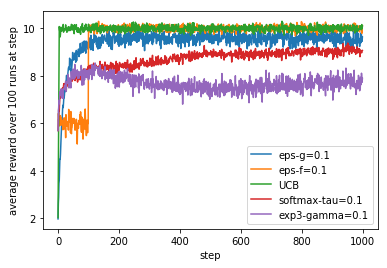
\includegraphics[width=1\linewidth]{figs/base5_1ts_1000step_5algos.png}
    \caption{Average reward over time for each algorithm over 1000 steps using the $base5$ peers with 1 time step per action.}
    \label{fig:base5_1ts_1000step_5algos}
\end{figure}

Figure \ref{fig:gen10_1ts_1000step_5algos} uses the dynamic $gen10$ peer set. Exp3 seems to peak higher than SoftMax compared to Figure \ref{fig:base5_1ts_1000step_5algos}, 
but then decays to below SoftMax's performance. The other algorithms have similar performance, althought it seems that UCB suffers slightly in the stochastic scenario. 
% gen10 peers. Timesteps=1
\begin{figure}[h]
    \centering
    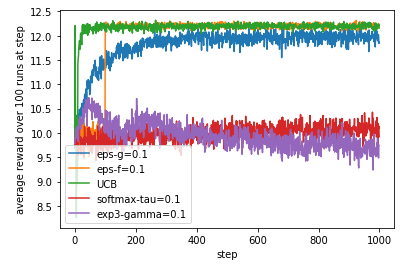
\includegraphics[width=1\linewidth]{figs/gen10_1ts_1000step_5algos.png}
    \caption{Average reward over time for each algorithm over 1000 steps using $gen10$ peers with 1 time step per action.}
    \label{fig:gen10_1ts_1000step_5algos}
\end{figure}

Cranking the time steps to 20 (the amount of time steps the agent will dedicate to a particular peer) shows a sufficient reduction in the variance of SoftMax and Exp3 in 
Figure \ref{fig:gen10_20ts_1000step_5algos}. However, it is also worth noting that the overall average reward peaks lower for each algorithm, compared to 
Figure \ref{fig:gen10_1ts_1000step_5algos}, with 1 time step per action.
% gen10 peers. Timesteps=20
\begin{figure}[h]
    \centering
    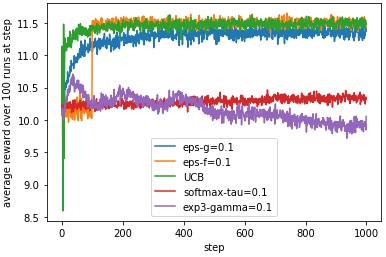
\includegraphics[width=1\linewidth]{figs/gen10_20ts_1000step_5algos.png}
    \caption{Average reward over time for each algorithm over 1000 steps using $gen10$ peers with 20 time steps per action.}
    \label{fig:gen10_20ts_1000step_5algos}
\end{figure}

% Then n=25 gen peers. (?)

Based on the results in Figure \ref{fig:base5_1ts_1000step_5algos}, we wanted to find out if SoftMax would ever overtake $\varepsilon$-greedy. In 
Figure \ref{fig:base5_1ts_40000step_eps_sm} we see that SoftMax eventually stabilizes higher than $\varepsilon$-greedy, and with lower variance.
% Does softmax eventually overtake eps-greedy? base5 peers case vs. n=10 gen peers case.
\begin{figure}[h]
    \centering
    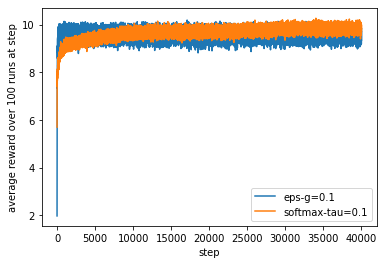
\includegraphics[width=1\linewidth]{figs/base5_1ts_40000step_eps-g_softmax.png}
    \caption{Average reward over time for $\varepsilon$-greedy and SoftMax over 40000 steps using $base5$ peers with 1 time step per action.}
    \label{fig:base5_1ts_40000step_eps_sm}
\end{figure}

However, Figure \ref{fig:gen10_1ts_20000step_eps_sm} show that this is not the case for the $gen10$ peers. Even after only 20000 steps, it is clear that SoftMax 
is not rising above $\varepsilon$-greedy like it was with $base5$. 
\begin{figure}[h]
    \centering
    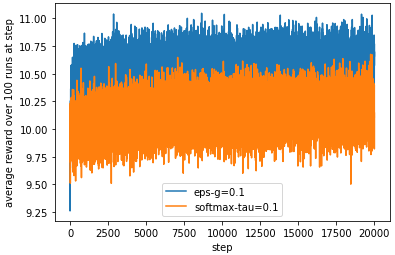
\includegraphics[width=1\linewidth]{figs/gen10_1ts_20000step_eps-g_softmax.png}
    \caption{Average reward over time for $\varepsilon$-greedy and SoftMax over 20000 steps using $gen10$ peers with 1 time step per action.}
    \label{fig:gen10_1ts_20000step_eps_sm}
\end{figure}

%-------------------------------------------------------------------------------
% Discussion on results. Pros and cons of suggested solution compared with existing solutions. 
\section{Discussion}

% UCB is insanely good. SoftMax and Exp3 have some interesting short/long term tradeoffs.
Based on our experiment results we found UCB to perform exceptionally well in each of our test scenarios. This was roughly what we had expected based on our research and 
findings from the related works, but were still surprised given the few amount of steps it required. Both $\varepsilon$-greedy and $\varepsilon$-forward performed well
but took many more steps to achieve UCBs performance. $\varepsilon$-forward seems to struggle in the first ~100 steps but then quickly jumps to oscillating around
the performance of UCB, while $\varepsilon$-greedy more gradually brought itself to under approximating UCB. SoftMax and Exp3 had a few interesting short term and long term
tradeoffs when compared to the other algorithms. To understand these tradeoffs we directly compared SoftMax to $\varepsilon$-greedy over a larger period of steps than before 
and altered the number of peers as seen in Figure\ref{fig:base5_1ts_40000step_eps_sm} and Figure\ref{fig:gen10_1ts_20000step_eps_sm}. We were able to identify that although 
SoftMax does start to rise above $\varepsilon$-greedy, if the number of peers are increased this does not occur. This does give some appeal to SoftMax if we were in a 
scenario where the number of peers was few and running for an extended time, but this is unlikely. 

% Not sure exactly what else we want to discuss here. Thought I would layout the main information. Unless we want to bring in more details.

%-------------------------------------------------------------------------------
% What we learned. Future work, takeaways.
\section{Conclusion and Future Research}

Conclusion: Simple summary of our findings, this may be similar to the discussion section but just more condensed.

What we learned: This could consist of the algorithms we implemented and the other ones discusses. Also should discuss how we had no prior RL experience
before this class and possibly additional stuff we learned from class.

Future Work: Probably just consists of how we could implement the POKER algorithm and some of the other algorithms in the related works such as the gossip algorithms. Could
also discuss how increasing the number of peers within the network may change the results of how the algorithm performs. Exploring an environment where there is more stochastic 
features may also be interesting.

\bibliography{refs}
\bibliographystyle{icml2021}

\end{document}